\section{Evaluation and Results}

\begin{figure*}[t]
    \centering
    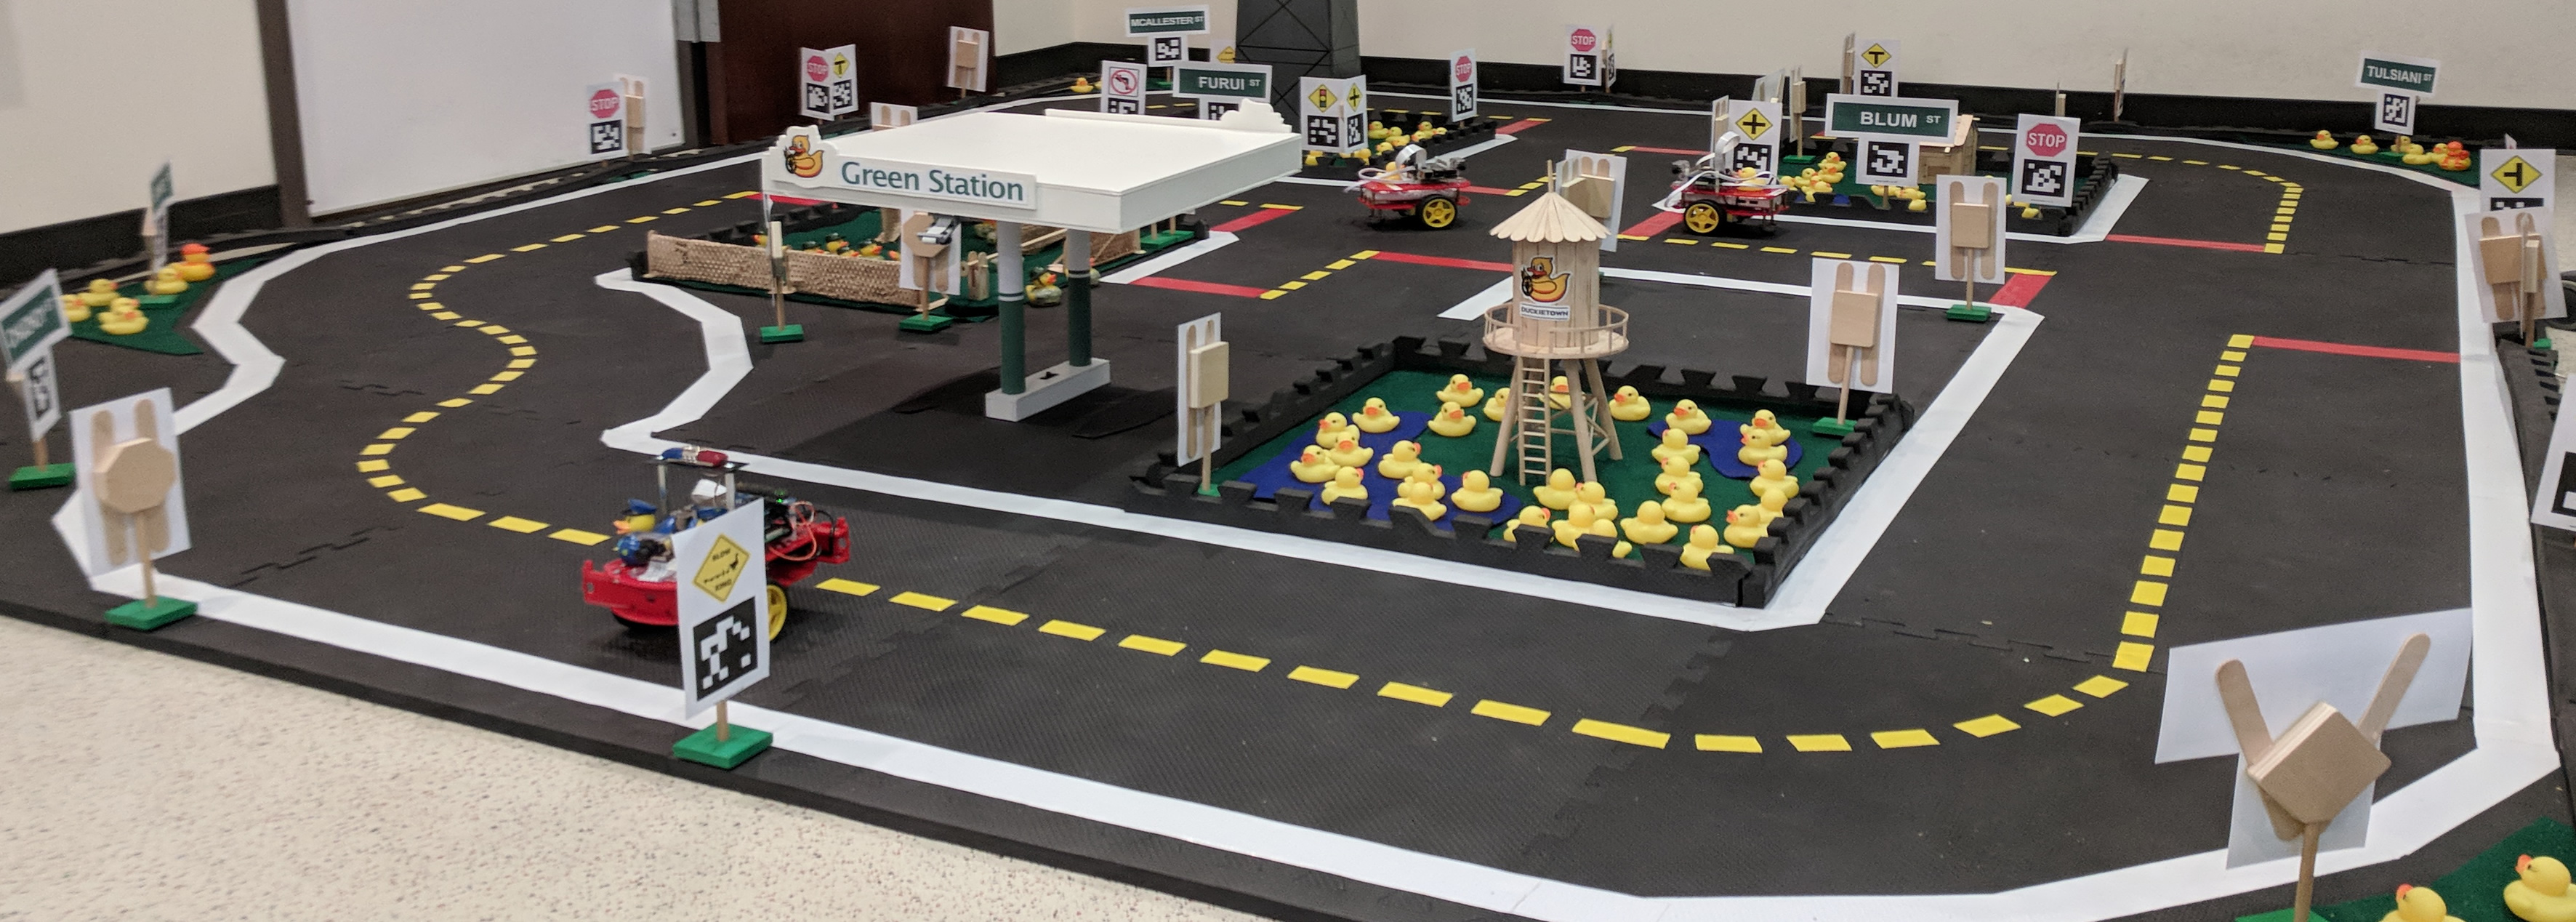
\includegraphics[width=\textwidth]{figures/duckietown.jpg}
    \vspace{-12pt}
    \caption{Duckietown at the Toyota Technological Institute at Chicago (TTIC) \label{fig:duckietown}}
\end{figure*}

\begin{figure}[t]
    \centering
    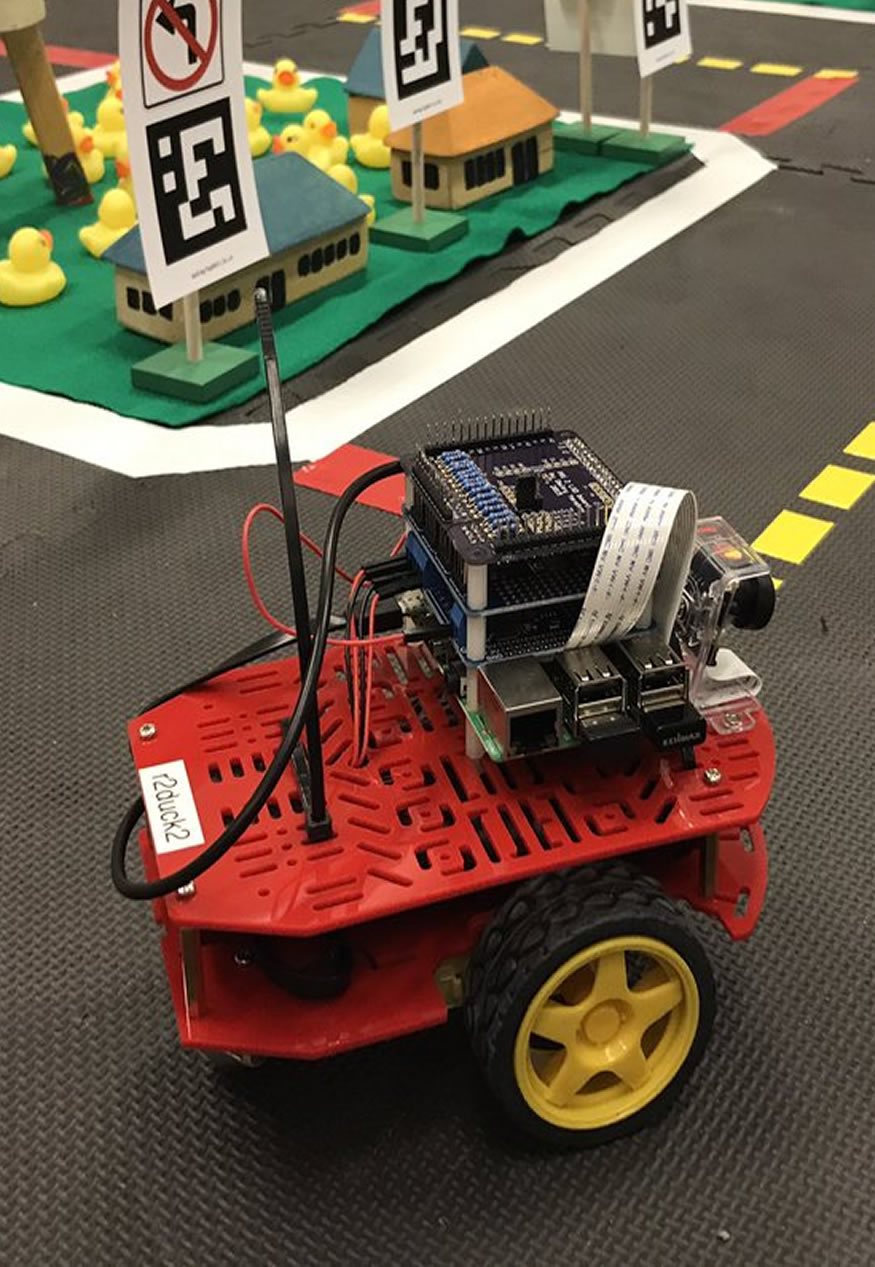
\includegraphics[width=0.48\textwidth]{figures/duckiebot.jpg}    
    \caption{Duckiebot robot \label{fig:duckiebot}}
\end{figure}

We evaluate our communication pipeline on a fleet of robots (i.e., Duckiebots) driving autonomously in a 
realistic model of a town called Duckietown~\cite{paull2017duckietown}. Figures~\ref{fig:duckietown} 
and~\ref{fig:duckiebot} show respectively our test-bed Duckietown, and one of the Duckiebots used in our 
experiments.
We test our communication pipeline on a common hazardous situations, that is a car accident at a 3-way 
intersection in the case of low visibility weather. For the remainder of this document we will refer to the location of
the accident (its GPS coordinates) as the \textit{Point of Interest} ($POI$). 
In our scenario, after the accident occurred, a number of 
vehicles $N$ will approach the same intersection from different directions and with different speed.
We test our model on a variable number of vehicles between $3$ and $6$. We observe consistent 
results across all the values of $N$ that we consider.
One experiment starts with $N$ vehicles start moving at the same time and from different locations and
driving towards the $POI$. The experiment ends when all the vehicles stop (either after they crashed
or stopped safely).
In our experiments, due to the lack of visibility, the first vehicle approaching the intersection will inevitably crash 
into the damaged vehicle. Immediately after the crash, the communication pipeline of such vehicle takes over.
We are interested in reducing the ratio $C$ of cars colliding with each other, as well as increasing 
the average distance $D_p$ from the $POI$ (how far away from the $POI$ a vehicle will stop) and the safety 
distance $D_s$, that is the average distance between two consecutive vehicles.

We evaluate the effectiveness of our pipeline by comparing the values of $C$, $D_p$, and $D_s$ 
with those achieved by the baseline.
In real life scenarios, when no autonomy is involved, 
the outcome of such an event heavily depends on the drivers' ability, experience, attention, and 
responsiveness~\todoad{Maybe cite something here?} as well as visibility conditions (e.g., lens flare at sunset and 
sunrise, fog, occlusions). This makes it hard to define
a baseline to compare against. Although, we can all agree on two points: (i) the worst case (i.e., all approaching 
cars crashing) is not unlikely to happen; (ii) the difference between worst and best case scenario is not a mere 
number when people's lives is involved. For these reason, we consider the worst case as a baseline.

\subsection{Technological and Physical limitations}
We are interested in the effect of our model in real life scenarios. In order to reduce the differences between 
our lab setup and the real world, we simulate physical effects such as wireless communication range limits, 
communication instability due to packets loss, and GPS-based localization latency.
We artificially simulate the wireless communication limit to $\wireless_limit_meter m$ (scaled to real world) by 
ignoring all the messages that are sent from a distance that is higher than the limit. Communication instability
is simulated by exchanging information via UDP protocol, that does not attempt re-transmission in case
of lost packets (unlike TCP). We also introduce a $\gps_delay_sec$ second delay between the GPS location 
we broadcast to the robots and their actual location.

\subsection{Ablation tests}
As explained in Section~\ref{sec:solution}, our communication pipeline implements three key features:
message propagation, message broadcasting, and reaction time aware communication.

We believe that these features are fundamental for improving self-driving vehicles' safety via explicit
communication. In order to study the contribution of each feature, we run an ablation test, in which we
run the same number of experiments on a version of our pipeline obtained by disabling one or multiple
features.
In particular, we consider four different models:

\begin{itemize}
\item \textbf{baseline}: No communication
\item \textbf{communication-only}: No propagation, No broadcasting
\item \textbf{propagation-only}: Propagation, No broadcasting
\item \textbf{full-pipeline}: Full communication pipeline
\end{itemize}

We run $\num_test_per_scenario$ tests for each communication model. For a given vehicle, initial position, 
speed, and direction are kept unchanged throughout all the tests.

\subsection{Results}

\begin{figure}[t]
    \centering
    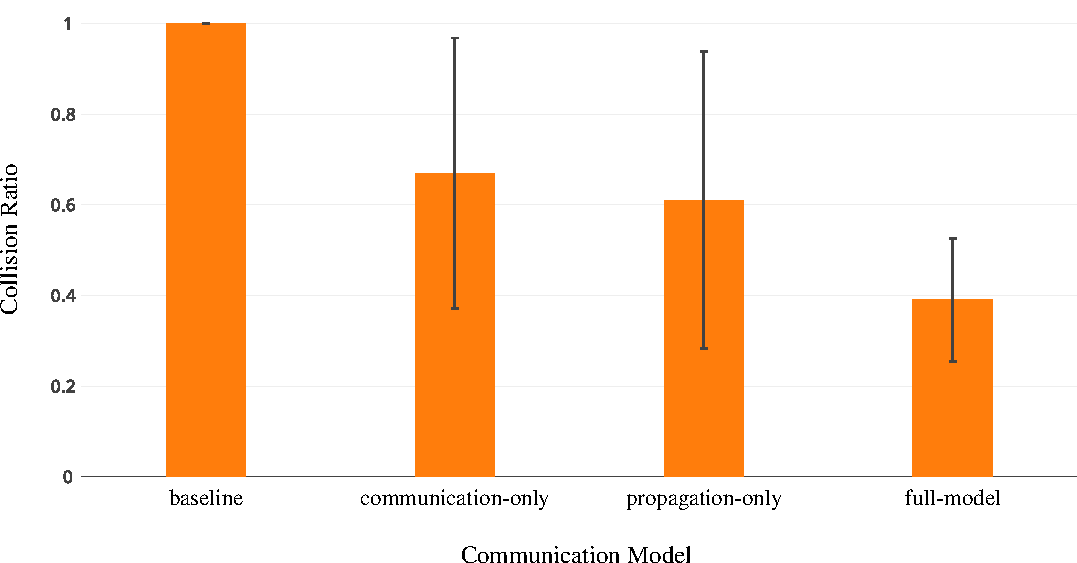
\includegraphics[width=0.48\textwidth, height=120px]{figures/collision_ratio.pdf}
    \caption{Collision ratio ($C$) for different communication models \label{fig:collision_ratio}}
\end{figure}

Figure~\ref{fig:collision_ratio} shows the collision ratio observed for different communication models in the
case of $N=3$ vehicles approaching the $POI$. We observe that in the absence of good visual perception
(\textbf{baseline}), as we consider the worst case, the collision rate is $100\%$ as all the vehicles will end up 
colliding with each other at the $POI$. By enabling the first vehicle that reaches the $POI$ (and collides) to
warn all the vehicles within the communication range (\textbf{communication-only}), we found out that on 
average, only one vehicle out of $3$ is close enough to receive the message and stop safely. It is worth noting
that any other vehicle entering the communication range after the message was sent will not receive any message
because the vehicle will not keep broadcasting the message. This means that whether the vehicles will collide or 
not, strictly depends on their position when the message was generated. A natural extension of this model
would be to allow all the vehicles that received the message to propagate it to other vehicles nearby 
(\textbf{propagation-only} model). We notice that even though the average collision ratio decreases,
the scenario can always degenerate to the case where all vehicles are too far from each other to exchange 
messages, hence they will all collide. 
Our complete communication pipeline (\textbf{full-model}) features all these communication strategies as well
as a broadcasting mechanism that allow all the vehicles that receive a message to keep publishing it at a frequency 
$F$. We empirically found that in our model of town, a frequency of $H=1Hz$ ensures safety while minimizing 
the load on the communication channel.

\begin{figure}[t]
    \centering
    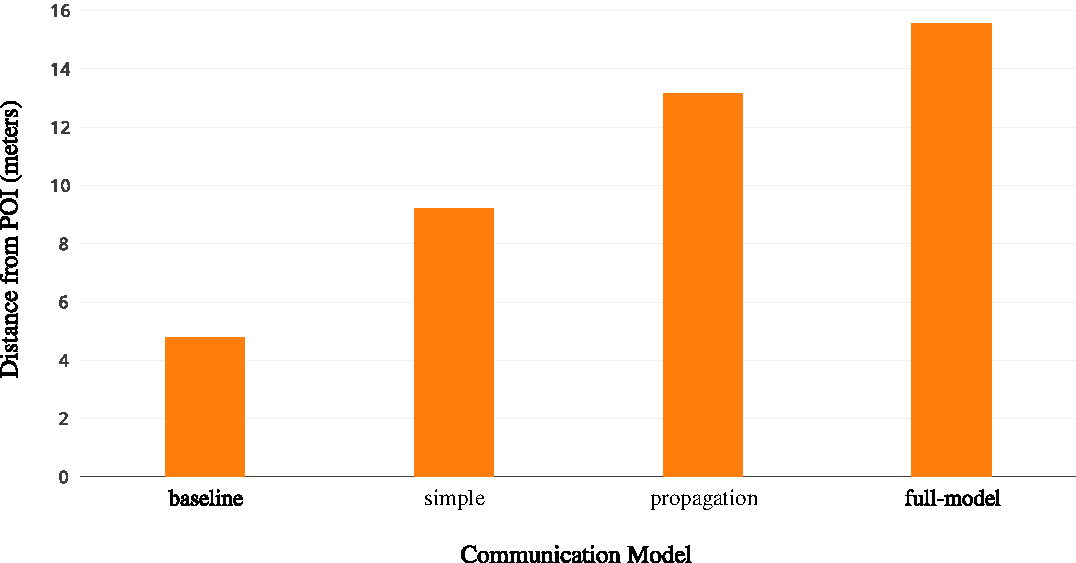
\includegraphics[width=0.48\textwidth, height=120px]{figures/distance_from_POI.pdf}
    \caption{Distance from the $POI$ ($D_p$) for different communication models \label{fig:distance_from_poi}}
\end{figure}

\begin{figure}[t]
    \centering
    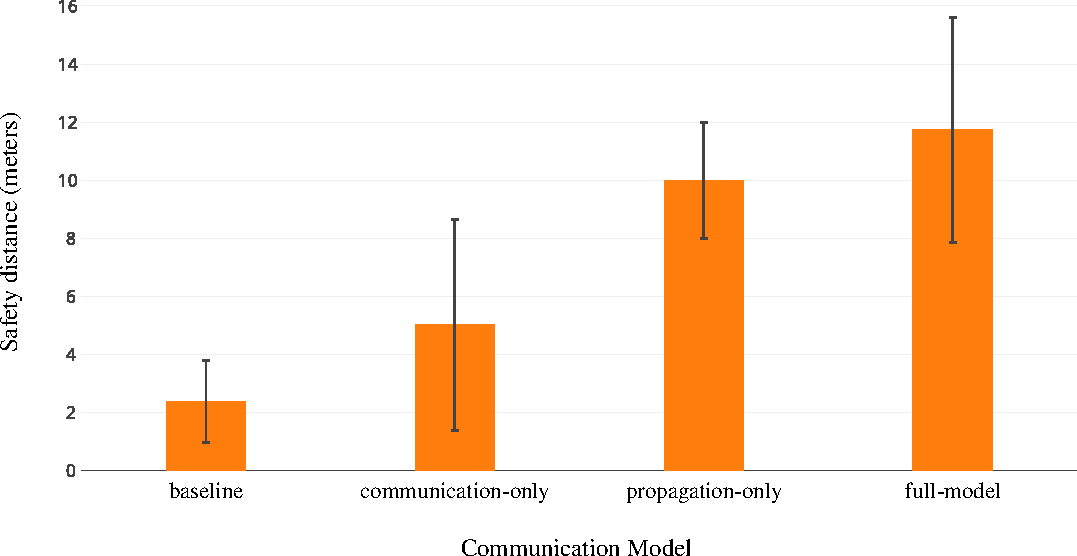
\includegraphics[width=0.48\textwidth, height=120px]{figures/safety_distance.pdf}
    \caption{Safety distance ($D_s$) between two consecutive vehicles \label{fig:safety_distance}}
\end{figure}

Figures~\ref{fig:distance_from_poi} and~\ref{fig:safety_distance} show the average distance 
between the $POI$ and the place where the vehicles stopped, and the average distance 
between two consecutive vehicles respectively (both scaled to the real world).
The distance $D_p$ is close to $4.5$ meters for the \textbf{baseline} model since all car collide with each 
other around the $POI$. The models \textbf{communication-only} and \textbf{propagation-only} increase both 
$D_p$ and $D_s$ compared to the baseline, but they fail when vehicles are outside the communication range(s).
The complete pipeline \textbf{full-model} succeed in warning vehicles that enter the communication range(s) later.
Unlike $D_p$, $D_s$ does not depend on the number of vehicles involved in the experiment, hence it 
is an absolute indicator of safety.

The proposed communication model achieves a collision ratio reduction of about $\collision_ratio_reduction_perc\%$,
while increasing the distance from the $POI$ and the safety distance between vehicles by a factor of 
$3$ and $5$ respectively, compared to the baseline.
